\documentclass{article}
\usepackage{amsmath}
\usepackage{amssymb}
\usepackage[dvipsnames]{xcolor}
\usepackage{graphicx}
\usepackage{enumitem}
\usepackage{centernot}
\usepackage{multicol}
\usepackage{forest}
\usepackage{bm}
\usepackage[margin=1.2in]{geometry}
\definecolor{light-gray}{gray}{0.95}
\newcommand{\code}[1]{\colorbox{light-gray}{\texttt{#1}}}
\begin{document}

\title{Algorithms Final Exam}
\author{Ozaner Hansha}
\date{May 12, 2020}
\maketitle

\subsection*{Problem 1}
Consider a recurrance relation of the form $T(n)=8T\left(\frac{n}{b}\right)+O(n^d)$ where $T(1)=1$.
\bigskip

\noindent\textbf{Part a:} Assign the smallest positive integer values to $b$ and $d$ so that $T(n)=O(n^3)$.
\bigskip

\noindent\textbf{Solution:} Call the $O(n^d)$ term in $T(n)$, $f(n)$. Now recall that:
$$f(n)=O(n^{\log_b 8-\epsilon})\implies T(n)=\Theta(n^{\log_b 8})$$

Where $\epsilon$ is some positive contant. We must have that $b=2$ so that $\log_2 8=3$ and thus $T(n)=\Theta(n^3)$. We must now pick a $d$ such that $O(n^d)=O(n^{\log_3 8-\epsilon})=O(n^{3-\epsilon})$. The smallest positive integer that satisfies this role is $d=1$. Thus our variables are $\bm{b=2}$ and $\bm{d=1}$.
\bigskip

\noindent\textbf{Part b:} Assign values to $b$ and $d$ so that $T(n)=O(n^2\log n)$.

\bigskip

\noindent\textbf{Solution:} Call the $O(n^d)$ term in $T(n)$, $f(n)$. Now recall that:
$$f(n)=\Theta(n^{\log_b 8})\implies T(n)=\Theta(n^{\log_b 8}\log n)$$

We must have that $b=2\sqrt{2}$ so that $\log_{2\sqrt{2}} 8=2$ and thus $T(n)=\Theta(n^2\log n)$. We must now pick a $d$ such that $O(n^d)=\Theta(n^{\log_{2\sqrt{2}} 8})=\Theta(n^2)$. We can simply pick $d=2$. Thus our variables are $\bm{b=2\sqrt{2}}$ and $\bm{d=2}$.

\subsection*{Problem 2}
\noindent\textbf{Problem:} Given an unsorted array $A$ of size $n$, give a linear time algorithm to output all elements between 80th and 90th percentile.
\bigskip

\noindent\textbf{Solution:} Let $k_1=\lfloor.8n\rfloor$ and $k_2=\lfloor.9n\rfloor$. We now perform the $k$th smallest element algorithm on the list $A$ for $k_1$, which takes $O(n)$ time. This nets us the 80th percentile $a_1$ of $A$. We now repeat this process for $k_2$, again taking $O(n)$ time, netting us the 90th precentile $a_2$ of $A$.

With these percentiles in hand, we now simply iterate through all $n$ elements of $A$ and print out the elements $a$ for which $a_1\le a\le a_2$. This iteration again takes $O(n)$ time.

This algorithm prints out all values of $A$ that fall in between its 80th and 90th percentile. And, as desired, the total complexity of the algorithm is given by $3\cdot O(n)=O(n)$.

% Recall that the $p$th percentile of a list $A$ is the smallest element $a_p$ in $A$ such that no more than $p\%$ of the data is less than $a_p$ and at least $p\%$ of the data is less than or equal to $a_p$.

\subsection*{Problem 3}
\noindent\textbf{Problem:} Do a DFS on the following graph starting at $A$, assuming vertices are considered in alphabetical order. Show discovery and finish times and classify edges as tree edges, forward edges, back edges, and cross edges.
\begin{center}
  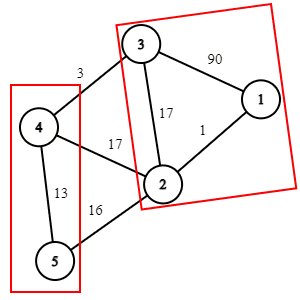
\includegraphics{graph3.png}
\end{center}

\noindent\textbf{Solution:} The discovery and finish times for each vertex are given below:
\begin{center}
  \begin{tabular}{c|c|c}
        Vertex & Discovery Time & Finished Time \\
        \hline
        $A$ & $1$ & $18$\\
        $B$ & $9$ & $12$\\
        $C$ & $2$ & $7$\\
        $D$ & $13$ & $14$\\
        $E$ & $8$ & $17$\\
        $F$ & $10$ & $11$\\
        $G$ & $4$ & $5$\\
        $H$ & $15$ & $16$\\
        $J$ & $3$ & $6$
  \end{tabular}
\end{center}
\medskip

Each of the edges is classified below:
\begin{center}
  \begin{tabular}{c|c|c|c}
        Tree Edges & Forward Edges & Cross Edges & Backward Edges \\
        \hline
        $(A,C),(C,J),(J,G),$ &  & $(D,C),(D,B),(H,B),$ & $(D,A)$\\
        $(A,E),(E,B),(B,F),$ & & $(H,F),(F,G),(B,J),$\\
        $(E,D),(E,H)$ & &
  \end{tabular}
\end{center}

\subsection*{Problem 4}
\noindent\textbf{Part a:} Compute the MST of the following graph using Kruskal’s algorithm. Show the order of the selected edges. If there is a tie, select edges in dictionary ordering, i.e. if you choose edge $(u, v)$, then $uv$ lexicographically precedes any other edge label $xy$:
\begin{center}
  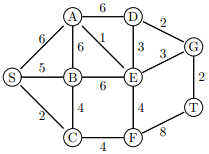
\includegraphics{graph4a.png}
\end{center}

\noindent\textbf{Solution:} The sets of spanned vertices and corresponding selected edge are given in the following table:
\begin{center}
\begin{tabular}{c|c|c|c}
  \textbf{Time} & \textbf{Selected} & &\\
  \textbf{Step} & \textbf{Edge} & \textbf{Added?} & \textbf{Sets of Spanned Vertices}\\
  \hline
  0 & - & - & $\{A\},\{B\},\{C\},\{D\},\{E\},\{F\},\{G\},\{S\},\{T\}$\\
  \hline
  1 & $(A,E)$ & Yes & $\{A,E\},\{B\},\{C\},\{D\},\{F\},\{G\},\{S\},\{T\}$\\
  \hline
  2 & $(C,S)$ & Yes & $\{A,E\},\{B\},\{C,S\},\{D\},\{F\},\{G\},\{T\}$\\
  \hline
  3 & $(D,G)$ & Yes & $\{A,E\},\{B\},\{C,S\},\{D,G\},\{F\},\{T\}$\\
  \hline
  4 & $(G,T)$ & Yes & $\{A,E\},\{B\},\{C,S\},\{D,G,T\},\{F\}$\\
  \hline
  5 & $(D,E)$ & Yes & $\{A,D,E,G,T\},\{B\},\{C,S\},\{F\}$\\
  \hline
  6 & $(E,G)$ & No & $\{A,D,E,G,T\},\{B\},\{C,S\},\{F\}$\\
  \hline
  7 & $(B,C)$ & Yes & $\{A,D,E,G,T\},\{B,C,S\},\{F\}$\\
  \hline
  8 & $(C,F)$ & Yes & $\{A,D,E,G,T\},\{B,C,F,S\}$\\
  \hline
  9 & $(E,F)$ & Yes & $\{A,B,C,D,E,F,G,S,T\}$
\end{tabular}
\end{center}
\smallskip

At step 9, all sets have been combined and our MST is complete:
\begin{center}
  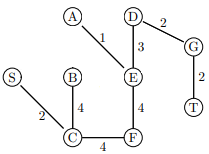
\includegraphics{graph4aMST.png}
\end{center}
\bigskip

\noindent\textbf{Part b:} Compute the MST of the following graph using Prim’s algorithm. Start at $S$ and give the order of the selected edges:
\begin{center}
  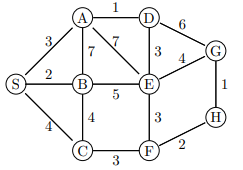
\includegraphics{graph4b.png}
\end{center}

\noindent\textbf{Solution:} Running Prim's algorithm starting at $S$ nets us:
\begin{center}
\begin{tabular}{c|c|c}
  \textbf{Order} & \textbf{Edge} & \textbf{Spanned Vertices}\\
  \hline
  1 & $(A,S)$ & $A,S$\\
  \hline
  2 & $(A,D)$ & $A,D,S$\\
  \hline
  3 & $(A,B)$ & $A,B,D,S$\\
  \hline
  4 & $(B,C)$ & $A,B,C,D,S$\\
  \hline
  5 & $(B,E)$ & $A,B,C,D,E,S$\\
  \hline
  6 & $(D,G)$ & $A,B,C,D,E,G,S$\\
  \hline
  7 & $(C,F)$ & $A,B,C,D,E,F,G,S$\\
  \hline
  8 & $(F,T)$ & $A,B,C,D,E,F,G,S,T$
\end{tabular}
\end{center}
\smallskip

At step 8, all vertices have been spanned and our MST is complete:
\begin{center}
  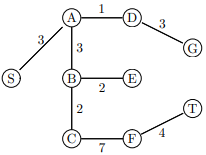
\includegraphics{graph4bMST.png}
\end{center}
\bigskip

\noindent\textbf{Part c:} Use Dijkstra’s algorithm to find the shortest path from $S$ to all other vertices.
\begin{center}
  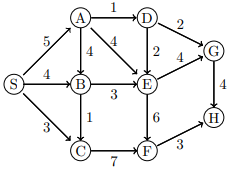
\includegraphics{graph4c.png}
\end{center}
\bigskip

\noindent\textbf{Solution:} Each iteration of Dijkstra’s algorithm is given below:
\bigskip

\hspace*{-0.4in}
\begin{tabular}{c|c|c|c|c|c|c|c|c|c}
  \textbf{Iteration} & $\bm{S}$ & $\bm{A}$ & $\bm{B}$ & $\bm{C}$ & $\bm{D}$ & $\bm{E}$ & $\bm{F}$ & $\bm{G}$ & $\bm{T}$\\\hline
  0 & 0, Null & $\infty$, Null & $\infty$, Null & $\infty$, Null & $\infty$, Null & $\infty$, Null & $\infty$, Null & $\infty$, Null & $\infty$, Null\\
  \hline
  1 & \textbf{0, Null} & 2, $S$ & 5, $S$ & 3, $S$ & $\infty$, Null & $\infty$, Null & $\infty$, Null & $\infty$, Null & $\infty$, Null\\
  \hline
  2 & - & $\bm{2, S}$ & 5, $S$ & 3, $S$ & 6, $A$ & 9, $A$ & $\infty$, Null & $\infty$, Null & $\infty$, Null\\
  \hline
  3 & - & - & 5, $S$ & $\bm{3, S}$ & 6, $A$ & 9, $A$ & 6, $C$ & $\infty$, Null & $\infty$, Null\\
  \hline
  4 & - & - & $\bm{5, S}$ & - & 6, $A$ & 7, $B$ & 6, $C$ & $\infty$, Null & $\infty$, Null\\
  \hline
  5 & - & - & - & - & $\bm{6, A}$ & 7, $B$ & 6, $C$ & 12, $D$ & $\infty$, Null\\
  \hline
  6 & - & - & - & - & - & 7, $B$ & $\bm{6, C}$ & 12, $D$ & 12, $F$\\
  \hline
  7 & - & - & - & - & - & $\bm{7, B}$ & - & 10, $E$ & 12, $F$\\
  \hline
  8 & - & - & - & - & - & - & - & $\bm{10, E}$ & 12, $F$\\
  \hline
  9 & - & - & - & - & - & - & - & - & $\bm{12, F}$
\end{tabular}
\bigskip

From this table we can construct the following shortest path tree with root $S$:
\begin{center}
  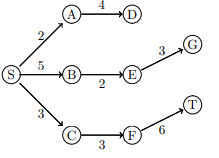
\includegraphics{graph4cSPT.png}
\end{center}

\noindent\textbf{Part d:} By inspection, find the shortest distance from $S$ to all other vertices, finite or infinite, in the following graph:
\begin{center}
  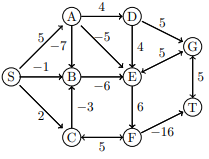
\includegraphics{graph4d.png}
\end{center}

\noindent\textbf{Solution:} By inspection, we find the following minimum distance paths from $S$ to all other vertices:
\begin{center}
  \begin{tabular}{c|c|l}
        Vertex & Min. Dist. & Min. Path \\
        \hline
        $A$ & $5$ & $SA$\\
        $B$ & $-2$ & $SAB$\\
        $C$ & $2$ & $SC$\\
        $D$ & $9$ & $SAD$\\
        $E$ & $-8$ & $SABE$\\
        $F$ & $-2$ & $SABEF$\\
        $G$ & $-13$ & $SABEFTG$\\
        $S$ & $0$ & -\\
        $T$ & $-18$ & $SABEFT$
  \end{tabular}
\end{center}

\subsection*{Problem 5}
\noindent\textbf{Problem:} For the patterns $AAAAAB$ and $ABABAC$, give $\operatorname{fail}(k)$ for each $k\in[1..6]$.
\bigskip

\noindent\textbf{Solution:} Running the KMP algorithm on both patterns we find:
\begin{center}
  \begin{tabular}{c|c|c|c|c|c|c}
        $k$&1&2&3&4&5&6 \\
        \hline
        Character&A&A&A&A&A&B\\
        \hline
        $\operatorname{fail}(k)$&0&1&2&3&4&5
  \end{tabular}\quad
  \begin{tabular}{c|c|c|c|c|c|c}
    $k$&1&2&3&4&5&6 \\
    \hline
    Character&A&B&A&B&A&C\\
    \hline
    $\operatorname{fail}(k)$&0&1&1&2&3&4
\end{tabular}
\end{center}


\subsection*{Problem 6}
\noindent\textbf{Part a:} Given a CNF formula on $n$ Boolean variables $x_1,\cdots,x_n$ and their negations with 5 clauses, describe a polynomial-time algorithm that would test if it is satisfiable.
\bigskip

\noindent\textbf{Solution:} First we construct the corresponding graph of the CNF, and check if a clique of size 5 exists. If so, then the CNF is satisfiable. If not, then the CNF isn't satisfiable. Note that for a fixed $k$, finding a $k$-clique in a graph takes only polynomial time.
\bigskip

\noindent\textbf{Part b:} Convert the following CNF to an equivalent 3-CNF formula:
$$(\overline{x_1}\vee x_2\vee x_3\vee \overline{x_4})\wedge(x_1\vee x_2\vee x_3\vee x_4\vee \overline{x_5})$$

\noindent\textbf{Solution:} We convert the above 5-CNF to a 3-CNF by introducing 3 new variables $q_1,q_2$, and $q3$:
$$(\overline{x_1}\vee x_2\vee q_1)\wedge(\overline{q_2}\vee x_3\vee \overline{x_4})\wedge(x_1\vee x_2\vee q_2)\wedge(\overline{q_2}\vee x_3\vee q_3)\wedge(\overline{q_3}\vee x_4\vee \overline{x_5})$$

\subsection*{Problem 7}
\noindent\textbf{Part a:} Given an undirected graph $G=(V, E)$, a subset of vertices $V'$ is an independent set if each edge in $E$ is incident to at most one vertex in $V'$. The independent set problem asks if $G$ has an independent set of size $k$. Find a maximal independent set in the undirected form of the graph from Problem 3.
\bigskip

\noindent\textbf{Solution:} The maximum size an independent set on this graph can be is 3. One such maximal independent set is $\{A,J,F\}$.
\bigskip

\noindent\textbf{Part b:} For a given graph $G$, consider $\overline{G}$, the complement graph of $\overline{G}$ (same vertices, complementary edges) and the clique problem. What relationship can you state between an independent set in $G$ and clique in $\overline{G}$? What can you conclude about the complexity class of independent set problem?
\bigskip

\noindent\textbf{Solution:} Given an independent set $S$ on some graph $G$, that same set $S$ is a clique on the complementary graph $\overline{G}$. This implies that the both the maximal and minimal indpendent set of $G$ equal the maximal and minimal clique in $\overline{G}$, respectively, and vice versa.

In terms of complexity, since constructing a graph $G$'s complement $\overline{G}$ takes polynomial time, we know that solving the independent set problem is in the same complexity class as the clique problem, and vice versa, up to some polynomial. In particular, since the independent set problem is in NP, we know the clique problem must also be in NP. If the clique problem was in, say, P, then we could easily convert it to an independent set problem in polynomial time and solve the independent set problem in polynomial time, causing a contradiction.

\subsection*{Problem 8}
Consider the following graph:
\begin{center}
  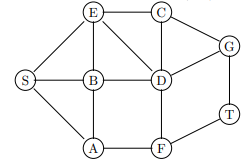
\includegraphics{graph8.png}
\end{center}

\noindent\textbf{Part a:} Give a maximal independent set of the graph.
\bigskip

\noindent\textbf{Solution:} This graph is essentially identical to that of Problem 7, and thus also has a maximal independent set of size 3. We present one such set below:
\begin{center}
  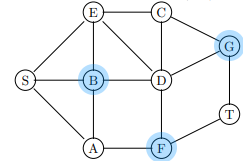
\includegraphics{graph8a.png}
\end{center}

\noindent\textbf{Part b:} Give a minimal vertex cover of the graph.
\bigskip

\noindent\textbf{Solution:} Recall from Problem 7 part b that the maximum clique size of this graph is equal to the maximum independent set size: 3. Now also recall that, for a max clique size of $k$, the size of the minimum vertex cover of a graph is $|V|-k$. As such we expect a minimum vertex cover size of $9-3=6$, and indeed that is what we find:
\begin{center}
  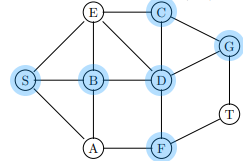
\includegraphics{graph8b.png}
\end{center}

\noindent\textbf{Part c:} Apply the vertex cover approximation algorithm described in lecture, using edges in dictionary ordering, i.e. if you choose edge $(u, v)$, then $uv$ lexicographically precedes any other edge label $xy$.
\bigskip

\noindent\textbf{Solution:} Starting with edge $(A,B)$, our cover set is now $\{A,B\}$ and the remaining edges are:
\begin{center}
  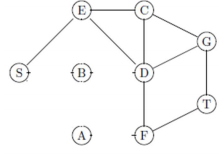
\includegraphics{graph8c-1.png}
\end{center}

Moving onto edge $(C,D)$, our cover set is now $\{A,B,C,D\}$ and the remaining edges are:
\begin{center}
  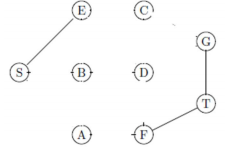
\includegraphics{graph8c-2.png}
\end{center}
\newpage

Moving onto edge $(E,S)$, our cover set is now $\{A,B,C,D,E,S\}$ and the remaining edges are:
\begin{center}
  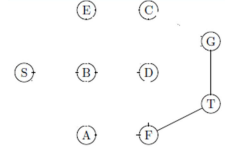
\includegraphics{graph8c-3.png}
\end{center}

Finally, we pick edge $(F,T)$, our cover set is now $\{A,B,C,D,E,F,S,T\}$ and there are no more remaining edges:
\begin{center}
  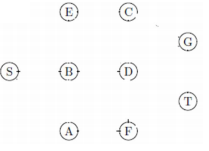
\includegraphics{graph8c-4.png}
\end{center}

This leaves us with the following cover set: $\bf{\{A,B,C,D,E,F,S,T\}}$.

\subsection*{Problem 9}
Consider the following directed graph:
\begin{center}
  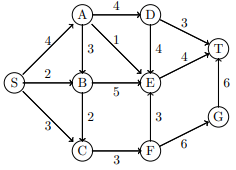
\includegraphics{graph9.png}
\end{center}
\medskip

\noindent\textbf{Part a:} Find the maximum flow from $S$ to $T$ by inspection.
\bigskip

\noindent\textbf{Solution:} The maximum flow from $S$ to $T$ is 9. Note that there is only $4+2+3=9$ capacity across all the outgoing edges of $S$, which means the flow cannot be any higher than 9. This, combined with the example below which has a total of 9 flow into the sink $T$, is sufficient to prove that 9 is the max flow:
\begin{center}
  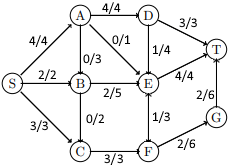
\includegraphics{graph9a.png}
\end{center}
\medskip

\noindent\textbf{Part b:} Give the residual graph corresponding to the optimal flow.
\bigskip

\noindent\textbf{Solution:} Below is the corresponding residual graph of the optimal solution given in part a:
\begin{center}
  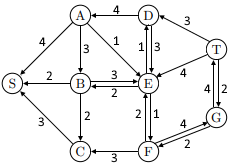
\includegraphics{graph9b.png}
\end{center}
\medskip

\noindent\textbf{Part c:} Give the minimum $(S,T)$ cut from the residual graph in part b.
\bigskip

\noindent\textbf{Solution:} The minimum cut is given by the following partition of $V$:
\begin{align*}
  L&=\{S\}\\
  R&=\{A,B,C,D,E,F,T,G\}
\end{align*}

Where $L$ is the set of vertices reachable from $S$ in the residual graph, and $R=L^\complement$. We can represent this graphically:
\begin{center}
  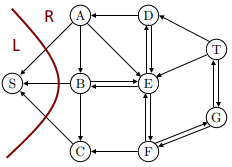
\includegraphics{graph9c.png}
\end{center}

\subsection*{Problem 10}
\noindent\textbf{Problem:} Using the shortest path algorithm for graphs, but via inspection, determine if the following system of inequalities has a feasible solution. If it has a feasible solution, find one. Otherwise, say why it is not feasible:
\begin{alignat*}{4}
  x_1-x_3&\le4  &\qquad  x_5-x_1&\le-2  &\qquad  x_1-x_2&\le3 &\qquad x_4-x_3&\le-2\\
  x_2-x_4&\le-3  &  x_3-x_2&\le8 &  x_4-x_5&\le2
\end{alignat*}

\noindent\textbf{Solution:} The corresponding graph of this system of inequalities is given by:
\begin{center}
  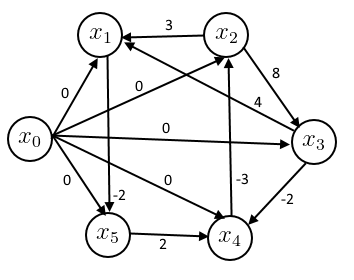
\includegraphics{graph10.png}
\end{center}

% Upon inspection, we note that there is indeed a negative cycle in this graph, namely $x_1x_5x_4x_2$ which nets -2 distance every time it is traveled through. This implies that the system of equations given above has no feasible solution.

Upon inspection, we note that there are no negative cycles and thus has a feasible solution. To calculate a solution, we proceed with the Bellman-Ford algorithm:
\begin{center}
  \begin{tabular}{c|c|c|c|c|c|c}
    \textbf{Iteration} & $\bm{x_0}$ & $\bm{x_1}$ & $\bm{x_2}$ & $\bm{x_3}$ & $\bm{x_4}$ & $\bm{x_5}$\\
    \hline
    0 & 0, Null & $\infty$, Null & $\infty$, Null & $\infty$, Null & $\infty$, Null & $\infty$, Null\\
    \hline
    1 & 0, Null & 0, $x_0$ & -5, $x_4$ & 0, $x_0$ & -2, $x_3$ & -2, $x_1$\\
    \hline
    2 & 0, Null & -2, $x_2$ & -5, $x_4$ & 0, $x_0$ & -2, $x_3$ & -2, $x_1$\\
    \hline
    3 & 0, Null & -2, $x_2$ & -5, $x_4$ & 0, $x_0$ & -2, $x_3$ & -4, $x_1$\\
    \hline
    4 & 0, Null & -2, $x_2$ & -5, $x_4$ & 0, $x_0$ & -2, $x_3$ & -4, $x_1$\\
    \hline
    5 & \textbf{0, Null} & $\bm{-2, x_2}$ & $\bm{-5, x_4}$ & $\bm{0, x_0}$ & $\bm{-2, x_3}$ & $\bm{-4, x_1}$
  \end{tabular}
\end{center}

And so a solution is given by the following assignment of variables:
\begin{alignat*}{3}
  x_1  & = -2  &\qquad  x_2 &  = -5  &\qquad  x_3  & = 0\\
  x_4  & = -2  &  x_5 & = -4
\end{alignat*}

\subsection*{Problem 11}
\noindent\textbf{Problem:} Are the following statements true or false?
\begin{enumerate}[label=\alph*)]
  \item To decide if a graph is 2-colorable is in P.
  \item In any complete graph with nonnegative weights on edges, the weight of any minimum spanning tree is no larger than the weight of any Hamiltonian cycle.  
  \item Computing the minimum vertex cover of a graph G that is a tree is solvable in polynomial time.
  \item To test if an integer n is not prime is in co-NP.
\end{enumerate}
\bigskip

\noindent\textbf{Solution:}
\begin{enumerate}[label=\alph*)]
  \item True
  \item True
  \item True
  \item True
\end{enumerate}

\end{document}